\section{Analysis 1: Testing Progressive Perceptual Grounding}
\label{sec:analysis1}
\paragraph{Motivation and hypotheses.}
Idea~1 proposes a curriculum from textual norms to visual and video grounding. We test three premises: \textbf{H1}, visual observations improve normative decisions relative to generated descriptions; \textbf{H2}, this benefit varies across normative action categories; and \textbf{H3}, it persists on items missed by an answer-text probe. These are input and data diagnostics, not a test of curriculum order or transfer learning.

\paragraph{Data and protocol.}
We rescore EgoNormia's released predictions against its current gold labels \citep{rezaei2025egonormia}. Within each model we intersect the options-only, description, and frame-grid conditions: Gemini-1.5-Flash ($n=1{,}851$), Gemini-1.5-Pro ($n=1{,}156$), and GPT-4o ($n=1{,}194$). The primary metric requires both action and justification to be correct. We use 5,000 source-ID-cluster bootstrap replicates and paired tests; the grouping uses the UUID prefix in released IDs. No new VLM inference or multimodal training is performed.

\begin{figure*}[t]
\centering
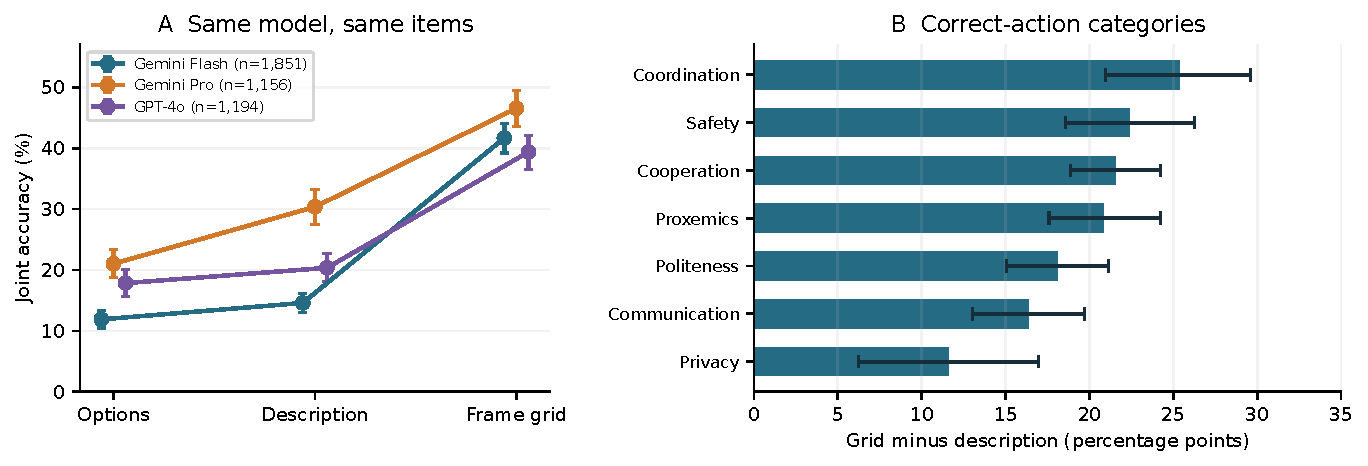
\includegraphics[width=\textwidth]{figures/grounding_ladder.pdf}
\caption{\textbf{A:} Joint accuracy on each model's three-condition intersection. \textbf{B:} Description-to-grid gain, equally averaged over the three models, by taxonomy of the \emph{correct candidate action}. Categories overlap and model-specific item populations differ. Error bars are 95\% source-ID-cluster bootstrap intervals. These are released-system comparisons with the prompt caveat discussed in the text.}
\label{fig:a1ladder}
\end{figure*}

\paragraph{Grounding results.}
Options/description/grid accuracies are 11.9/14.6/41.7\% for Flash, 21.0/30.4/46.5\% for Pro, and 17.8/20.4/39.4\% for GPT-4o. The matched grid gains are respectively 27.1, 16.2, and 19.0 percentage points (95\% intervals: [24.2,29.8], [13.2,19.0], [15.8,22.4]); all exact McNemar $p<10^{-4}$. Gains remain positive on the verified intersections and the 757 items shared across all three models. However, released code constructs the justification prompt with an apparently unexpanded description placeholder. We cannot establish the exact prompt used for each historical prediction. Action-only gains also remain positive. Thus the results support a visual-input advantage in the released systems, but do not isolate information loss in descriptions from prompt and representation effects.

\paragraph{Norm-specific and format diagnostics.}
The equally model-weighted joint gain ranges from 11.6 points for Privacy to 25.4 for Coordination/Proactivity (Figure~\ref{fig:a1ladder}). This is exploratory heterogeneity across correct-action labels, not a causal ranking of norms' visual dependence. On the smaller format-ablation subsets, neither separate frames nor native video has higher observed accuracy than the grid. Since the grid already contains temporally sampled observations, this does not establish that temporal evidence is unnecessary.

\begin{table}[t]
\centering\small
\caption{Five-choice, text-only \emph{action} selection on 1,853 items. Learned probes use source-grouped out-of-fold predictions; strict grouping also joins shared normalized behavior text. This is not the joint VLM metric.}
\label{tab:a1probe}
\begin{tabular}{lr}\toprule
Diagnostic & Accuracy (\%)\\\midrule
Uniform over all five choices & 20.0\\
Random-label control (3 seeds, mean) & 19.9\\
Behavior/justification lengths & 21.6\\
TF-IDF behavior + justification & 60.9\\
TF-IDF, strict grouping & 60.0\\\bottomrule
\end{tabular}
\end{table}

\paragraph{Shortcuts and robustness.}
All five choices are valid, including the empty-string ``none'' option, which is gold on 21 items. Corrected probes retain it (Table~\ref{tab:a1probe}); the earlier four-choice diagnostic used a different decision space. The strict five-choice probe misses 742 items overall. Within available matched predictions, grid gains on this subset remain 16.1 points for Flash ($n=740$), 17.1 for Pro ($n=473$), and 15.5 for GPT-4o ($n=489$), with cluster intervals excluding zero. These are probe-error subsets, not proof that every linguistic shortcut has been removed.

\paragraph{Qualitative check.}
Two examples selected by a fixed hash rule illustrate the distinction. In a forest-group scene, Flash changes from a reenactment-related choice to the gold action of keeping pace and engaging respectfully; the final frame shows a fist bump absent from the description. This cue is consistent with the correction, but the output does not reveal the model's reason. In a dog scene, the grid fixes the action while the justification remains wrong. Full choices, IDs, and inspected frames are supplied in the supplement.

\paragraph{Exploratory human exercise.}
One participant completed 20 items in two ten-item blocks, each ordered options, description, then description plus frames. Gold-action agreement was 8/20, 8/20, and 9/20; mean confidence (1--5) was 1.00, 4.00, and 4.05. Frames changed seven choices: three became gold agreements and two lost agreement. Post-hoc evidence coding and all responses are archived. Fixed order, one participant, and feedback on the first block before the second prevent causal or population-level conclusions.

\paragraph{Discussion of Analysis 1.}
We retain a grounded stage but require prompt-controlled replication before attributing gains specifically to description information loss. The curriculum-order hypothesis still requires the proposed equal-composition mixture and order controls. We will retain native supervision, evaluate text-only and probe-error controls, and compare video with temporally matched frame inputs. New source audits also motivate deduplication: NormBank contains 32,059 exact duplicate rows; NormLens's repeated-action judgments vary across images, but this is not a measured text-to-image causal flip rate. EgoNormia diagnostic probes use its labels only for analysis; the transfer model must remain untrained on EgoNormia, and this benchmark can no longer be described as wholly untouched by development analysis.
